% Options for packages loaded elsewhere
\PassOptionsToPackage{unicode}{hyperref}
\PassOptionsToPackage{hyphens}{url}
%
\documentclass[
  ignorenonframetext,
  aspectratio=169]{beamer}
\usepackage{pgfpages}
\setbeamertemplate{caption}[numbered]
\setbeamertemplate{caption label separator}{: }
\setbeamercolor{caption name}{fg=normal text.fg}
\beamertemplatenavigationsymbolsempty
% Prevent slide breaks in the middle of a paragraph
\widowpenalties 1 10000
\raggedbottom
\setbeamertemplate{part page}{
  \centering
  \begin{beamercolorbox}[sep=16pt,center]{part title}
    \usebeamerfont{part title}\insertpart\par
  \end{beamercolorbox}
}
\setbeamertemplate{section page}{
  \centering
  \begin{beamercolorbox}[sep=12pt,center]{part title}
    \usebeamerfont{section title}\insertsection\par
  \end{beamercolorbox}
}
\setbeamertemplate{subsection page}{
  \centering
  \begin{beamercolorbox}[sep=8pt,center]{part title}
    \usebeamerfont{subsection title}\insertsubsection\par
  \end{beamercolorbox}
}
\AtBeginPart{
  \frame{\partpage}
}
\AtBeginSection{
  \ifbibliography
  \else
    \frame{\sectionpage}
  \fi
}
\AtBeginSubsection{
  \frame{\subsectionpage}
}
\usepackage{amsmath,amssymb}
\usepackage{lmodern}
\usepackage{iftex}
\ifPDFTeX
  \usepackage[T1]{fontenc}
  \usepackage[utf8]{inputenc}
  \usepackage{textcomp} % provide euro and other symbols
\else % if luatex or xetex
  \usepackage{unicode-math}
  \defaultfontfeatures{Scale=MatchLowercase}
  \defaultfontfeatures[\rmfamily]{Ligatures=TeX,Scale=1}
\fi
% Use upquote if available, for straight quotes in verbatim environments
\IfFileExists{upquote.sty}{\usepackage{upquote}}{}
\IfFileExists{microtype.sty}{% use microtype if available
  \usepackage[]{microtype}
  \UseMicrotypeSet[protrusion]{basicmath} % disable protrusion for tt fonts
}{}
\makeatletter
\@ifundefined{KOMAClassName}{% if non-KOMA class
  \IfFileExists{parskip.sty}{%
    \usepackage{parskip}
  }{% else
    \setlength{\parindent}{0pt}
    \setlength{\parskip}{6pt plus 2pt minus 1pt}}
}{% if KOMA class
  \KOMAoptions{parskip=half}}
\makeatother
\usepackage{xcolor}
\newif\ifbibliography
\usepackage{color}
\usepackage{fancyvrb}
\newcommand{\VerbBar}{|}
\newcommand{\VERB}{\Verb[commandchars=\\\{\}]}
\DefineVerbatimEnvironment{Highlighting}{Verbatim}{commandchars=\\\{\}}
% Add ',fontsize=\small' for more characters per line
\usepackage{framed}
\definecolor{shadecolor}{RGB}{248,248,248}
\newenvironment{Shaded}{\begin{snugshade}}{\end{snugshade}}
\newcommand{\AlertTok}[1]{\textcolor[rgb]{0.94,0.16,0.16}{#1}}
\newcommand{\AnnotationTok}[1]{\textcolor[rgb]{0.56,0.35,0.01}{\textbf{\textit{#1}}}}
\newcommand{\AttributeTok}[1]{\textcolor[rgb]{0.77,0.63,0.00}{#1}}
\newcommand{\BaseNTok}[1]{\textcolor[rgb]{0.00,0.00,0.81}{#1}}
\newcommand{\BuiltInTok}[1]{#1}
\newcommand{\CharTok}[1]{\textcolor[rgb]{0.31,0.60,0.02}{#1}}
\newcommand{\CommentTok}[1]{\textcolor[rgb]{0.56,0.35,0.01}{\textit{#1}}}
\newcommand{\CommentVarTok}[1]{\textcolor[rgb]{0.56,0.35,0.01}{\textbf{\textit{#1}}}}
\newcommand{\ConstantTok}[1]{\textcolor[rgb]{0.00,0.00,0.00}{#1}}
\newcommand{\ControlFlowTok}[1]{\textcolor[rgb]{0.13,0.29,0.53}{\textbf{#1}}}
\newcommand{\DataTypeTok}[1]{\textcolor[rgb]{0.13,0.29,0.53}{#1}}
\newcommand{\DecValTok}[1]{\textcolor[rgb]{0.00,0.00,0.81}{#1}}
\newcommand{\DocumentationTok}[1]{\textcolor[rgb]{0.56,0.35,0.01}{\textbf{\textit{#1}}}}
\newcommand{\ErrorTok}[1]{\textcolor[rgb]{0.64,0.00,0.00}{\textbf{#1}}}
\newcommand{\ExtensionTok}[1]{#1}
\newcommand{\FloatTok}[1]{\textcolor[rgb]{0.00,0.00,0.81}{#1}}
\newcommand{\FunctionTok}[1]{\textcolor[rgb]{0.00,0.00,0.00}{#1}}
\newcommand{\ImportTok}[1]{#1}
\newcommand{\InformationTok}[1]{\textcolor[rgb]{0.56,0.35,0.01}{\textbf{\textit{#1}}}}
\newcommand{\KeywordTok}[1]{\textcolor[rgb]{0.13,0.29,0.53}{\textbf{#1}}}
\newcommand{\NormalTok}[1]{#1}
\newcommand{\OperatorTok}[1]{\textcolor[rgb]{0.81,0.36,0.00}{\textbf{#1}}}
\newcommand{\OtherTok}[1]{\textcolor[rgb]{0.56,0.35,0.01}{#1}}
\newcommand{\PreprocessorTok}[1]{\textcolor[rgb]{0.56,0.35,0.01}{\textit{#1}}}
\newcommand{\RegionMarkerTok}[1]{#1}
\newcommand{\SpecialCharTok}[1]{\textcolor[rgb]{0.00,0.00,0.00}{#1}}
\newcommand{\SpecialStringTok}[1]{\textcolor[rgb]{0.31,0.60,0.02}{#1}}
\newcommand{\StringTok}[1]{\textcolor[rgb]{0.31,0.60,0.02}{#1}}
\newcommand{\VariableTok}[1]{\textcolor[rgb]{0.00,0.00,0.00}{#1}}
\newcommand{\VerbatimStringTok}[1]{\textcolor[rgb]{0.31,0.60,0.02}{#1}}
\newcommand{\WarningTok}[1]{\textcolor[rgb]{0.56,0.35,0.01}{\textbf{\textit{#1}}}}
\usepackage{longtable,booktabs,array}
\usepackage{calc} % for calculating minipage widths
\usepackage{caption}
% Make caption package work with longtable
\makeatletter
\def\fnum@table{\tablename~\thetable}
\makeatother
\setlength{\emergencystretch}{3em} % prevent overfull lines
\providecommand{\tightlist}{%
  \setlength{\itemsep}{0pt}\setlength{\parskip}{0pt}}
\setcounter{secnumdepth}{-\maxdimen} % remove section numbering
%\usepackage[dct]{../../inst/rmarkdown/templates/autbeamer/skeleton/AUTtheme}     % AUT theme
\usepackage[dct]{AUTtheme}     % AUT theme


% Customise additional Beamer properties without changing AUTTheme.sty
%\setbeamerfont{title}{ series=\bfseries , size ={\fontsize{30}{30}}}
%\setbeamerfont{subtitle}{size ={\fontsize{13}{13}}}
%\setbeamerfont{author}{size = {\fontsize{11}{11}}}
%\setbeamerfont{date}{size = {\fontsize{11}{11}}}
%\setbeamerfont{institute}{size={\fontsize{11}{11}}}

\AtBeginSubsection[]{}

\AtBeginSection{
\begin{sectionframe}
\frametitle{Outline}
\tableofcontents[
    	currentsection,
        sectionstyle=show/shaded,
        subsectionstyle=show/show/hide,
    ]
\end{sectionframe}}



\ifLuaTeX
  \usepackage{selnolig}  % disable illegal ligatures
\fi
\IfFileExists{bookmark.sty}{\usepackage{bookmark}}{\usepackage{hyperref}}
\IfFileExists{xurl.sty}{\usepackage{xurl}}{} % add URL line breaks if available
\urlstyle{same} % disable monospaced font for URLs
\hypersetup{
  pdfauthor={Sarah Marshall},
  hidelinks,
  pdfcreator={LaTeX via pandoc}}

\title{Introduction to the AUTtheme\\
for R Markdown with Beamer}
\author{Sarah Marshall}
\date{24 February 2023}
\institute{Department of Mathematical Sciences\\
Auckland University of Technology}

\begin{document}
\frame{\titlepage}

\begin{frame}{Overview}
\protect\hypertarget{overview}{}
\tableofcontents[hideallsubsections]
\end{frame}

\hypertarget{usage}{%
\section{Usage}\label{usage}}

\hypertarget{how-to-load-this-package}{%
\subsection{How to load this package}\label{how-to-load-this-package}}

\begin{frame}[fragile]{How to load this package}
Load this package from github using the \texttt{remotes} package

In R Studio

\begin{itemize}
\tightlist
\item
  File/New File/R Markdown/From Template
\item
  Select AUTBeamer
\end{itemize}

This will create a new directory containing the required files to run
the template

\begin{itemize}
\tightlist
\item
  bgImages (folder containing images)
\item
  AUTtheme.sty
\item
  header.tex
\item
  untitled.Rmd
\end{itemize}
\end{frame}

\hypertarget{compiling-this-demo-file}{%
\subsection{Compiling this demo file}\label{compiling-this-demo-file}}

\begin{frame}[fragile]{Compiling this demo file}
To compile this demo file, this file needs to be located in the same
directory as the \texttt{bgImages} folder and the \texttt{AUTtheme.sty}
file. These files are not provided in the demo folder to avoid
duplication.
\end{frame}

\hypertarget{compiling-with-auttheme}{%
\subsection{Compiling with AUTTheme}\label{compiling-with-auttheme}}

\begin{frame}[fragile]{Compiling with AUTTheme}
\texttt{lualatex} is recommended.
\end{frame}

\hypertarget{comparison-to-beamer-version}{%
\subsection{Comparison to Beamer
version}\label{comparison-to-beamer-version}}

\begin{frame}{Comparison to Beamer version}
The Rmd version of this template does not yet have all the functionality
of the beamer version, e.g.~customised frame environments such as
sectionpages.
\end{frame}

\hypertarget{frames}{%
\section{Frames}\label{frames}}

\hypertarget{frame-sizes}{%
\subsection{Frame Sizes}\label{frame-sizes}}

\begin{frame}[fragile]{Frame Sizes}
The template can be used to create \(16\times9\) or \(4 \times 3\)
slides by modifying the YAML header.

The resolution of the background images get updated automatically.

\begin{itemize}
\tightlist
\item
  To create \(16 \times 9\) slides use
  \texttt{classoption:\ "aspectratio=169"}
\item
  To create \(4 \times 3\) slides use
  \texttt{classoption:\ "aspectratio=43"}
\end{itemize}
\end{frame}

\hypertarget{customisation}{%
\subsection{Customisation}\label{customisation}}

\begin{frame}[fragile]{Customisation}
The file \texttt{header.tex} contains the LaTeX commands used at the
start of the document.

To use the AUTtheme package, \texttt{header.tex} needs to contain, a
command like:

\begin{itemize}
\tightlist
\item
  \texttt{\textbackslash{}usepackage\{AUTtheme\}} or
\item
  \texttt{\textbackslash{}usepackage{[}dct{]}\{AUTtheme\}}
\end{itemize}

The \texttt{header.tex} file can also be used to load other packages or
customise the Beamer package in other ways, e.g.

\texttt{\textbackslash{}AtBeginSection\{\}}

or

\texttt{usepackage\{lipsum\}}
\end{frame}

\hypertarget{outlines}{%
\subsection{Outlines}\label{outlines}}

\begin{frame}[fragile]{Outlines}
Sections are defined by \texttt{\#}, subsections by \texttt{\#\#} and
slides by \texttt{\#\#\#}. The \texttt{slide\_level} can be defined in
the YAML header.

An outline of all sections can be created by adding:

\texttt{\textbackslash{}tableofcontents{[}hideallsubsections{]}}
\end{frame}

\begin{frame}{Overview - Example 1}
\protect\hypertarget{overview---example-1}{}
\tableofcontents[hideallsubsections]
\end{frame}

\begin{frame}{Overview - Example 2}
\protect\hypertarget{overview---example-2}{}
\tableofcontents[
        currentsection,
      sectionstyle=show/shaded,
      subsectionstyle = hide/hide/hide
    ]
\end{frame}

\begin{frame}{Overview - Example 3}
\protect\hypertarget{overview---example-3}{}
\tableofcontents[
        currentsection,
      sectionstyle=show/shaded,
      subsectionstyle=show/shaded/hide
    ]
\end{frame}

\hypertarget{atbeginsection}{%
\subsection{\texorpdfstring{\texttt{\textbackslash{}AtBeginSection}}{\textbackslash AtBeginSection}}\label{atbeginsection}}

\begin{frame}[fragile]{\texttt{\textbackslash{}AtBeginSection}}
In \texttt{AUTtheme.sty} the default is that each section starts:

\begin{itemize}
\tightlist
\item
  with a title slide containing the section name
\item
  an outline slide with the following specification
\end{itemize}

\begin{Shaded}
\begin{Highlighting}[]
\NormalTok{\textbackslash{}tableofcontents[}
\NormalTok{      currentsubsection,}
\NormalTok{      sectionstyle}\OtherTok{=}\NormalTok{show}\SpecialCharTok{/}\NormalTok{shaded,}
\NormalTok{      subsectionstyle}\OtherTok{=}\NormalTok{show}\SpecialCharTok{/}\NormalTok{shaded}\SpecialCharTok{/}\NormalTok{hide,}
\NormalTok{    ]}
\end{Highlighting}
\end{Shaded}
\end{frame}

\hypertarget{customising-atbeginsection}{%
\subsection{\texorpdfstring{Customising
\texttt{\textbackslash{}AtBeginSection}}{Customising \textbackslash AtBeginSection}}\label{customising-atbeginsection}}

\begin{frame}[fragile]{Customising
\texttt{\textbackslash{}AtBeginSection}}
This can be customised in \texttt{header.tex}. For example, as shown in
the header file for this demo

\begin{Shaded}
\begin{Highlighting}[]
\NormalTok{\textbackslash{}AtBeginSection\{}
\NormalTok{\textbackslash{}begin\{sectionframe\}}
\NormalTok{\textbackslash{}frametitle\{Outline\}}
\NormalTok{\textbackslash{}tableofcontents[}
\NormalTok{        currentsection,}
\NormalTok{        sectionstyle}\OtherTok{=}\NormalTok{show}\SpecialCharTok{/}\NormalTok{shaded,}
\NormalTok{        subsectionstyle}\OtherTok{=}\NormalTok{show}\SpecialCharTok{/}\NormalTok{show}\SpecialCharTok{/}\NormalTok{hide,}
\NormalTok{    ]}
\NormalTok{\textbackslash{}end\{sectionframe\}\}}
\end{Highlighting}
\end{Shaded}
\end{frame}

\hypertarget{common-frame-features-and-layouts}{%
\section{Common Frame Features and
Layouts}\label{common-frame-features-and-layouts}}

\hypertarget{lists}{%
\subsection{Lists}\label{lists}}

\begin{frame}{Unordered list}
\protect\hypertarget{unordered-list}{}
\begin{itemize}
\tightlist
\item
  Bullet 1

  \begin{itemize}
  \tightlist
  \item
    sub Bullet

    \begin{itemize}
    \tightlist
    \item
      sub of sub Bullet
    \end{itemize}
  \item
    sub Bullet
  \end{itemize}
\item
  Bullet 2
\item
  Bullet 3
\end{itemize}
\end{frame}

\begin{frame}{Ordered list}
\protect\hypertarget{ordered-list}{}
\begin{enumerate}
\tightlist
\item
  Item 1

  \begin{itemize}
  \tightlist
  \item
    Item 1a
  \item
    Item 1b
  \end{itemize}
\item
  Item 2
\item
  Item 3

  \begin{itemize}
  \tightlist
  \item
    Item 3a
  \item
    Item 3b
  \end{itemize}
\end{enumerate}
\end{frame}

\begin{frame}{List with steps showing}
\protect\hypertarget{list-with-steps-showing}{}
\begin{enumerate}[<+->]
\tightlist
\item
  Item 1
\item
  Item 2
\item
  Item 3
\end{enumerate}
\end{frame}

\hypertarget{columns}{%
\subsection{Columns}\label{columns}}

\begin{frame}{Columns}
\begin{columns}[T]
\begin{column}{0.6\textwidth}
Column 1

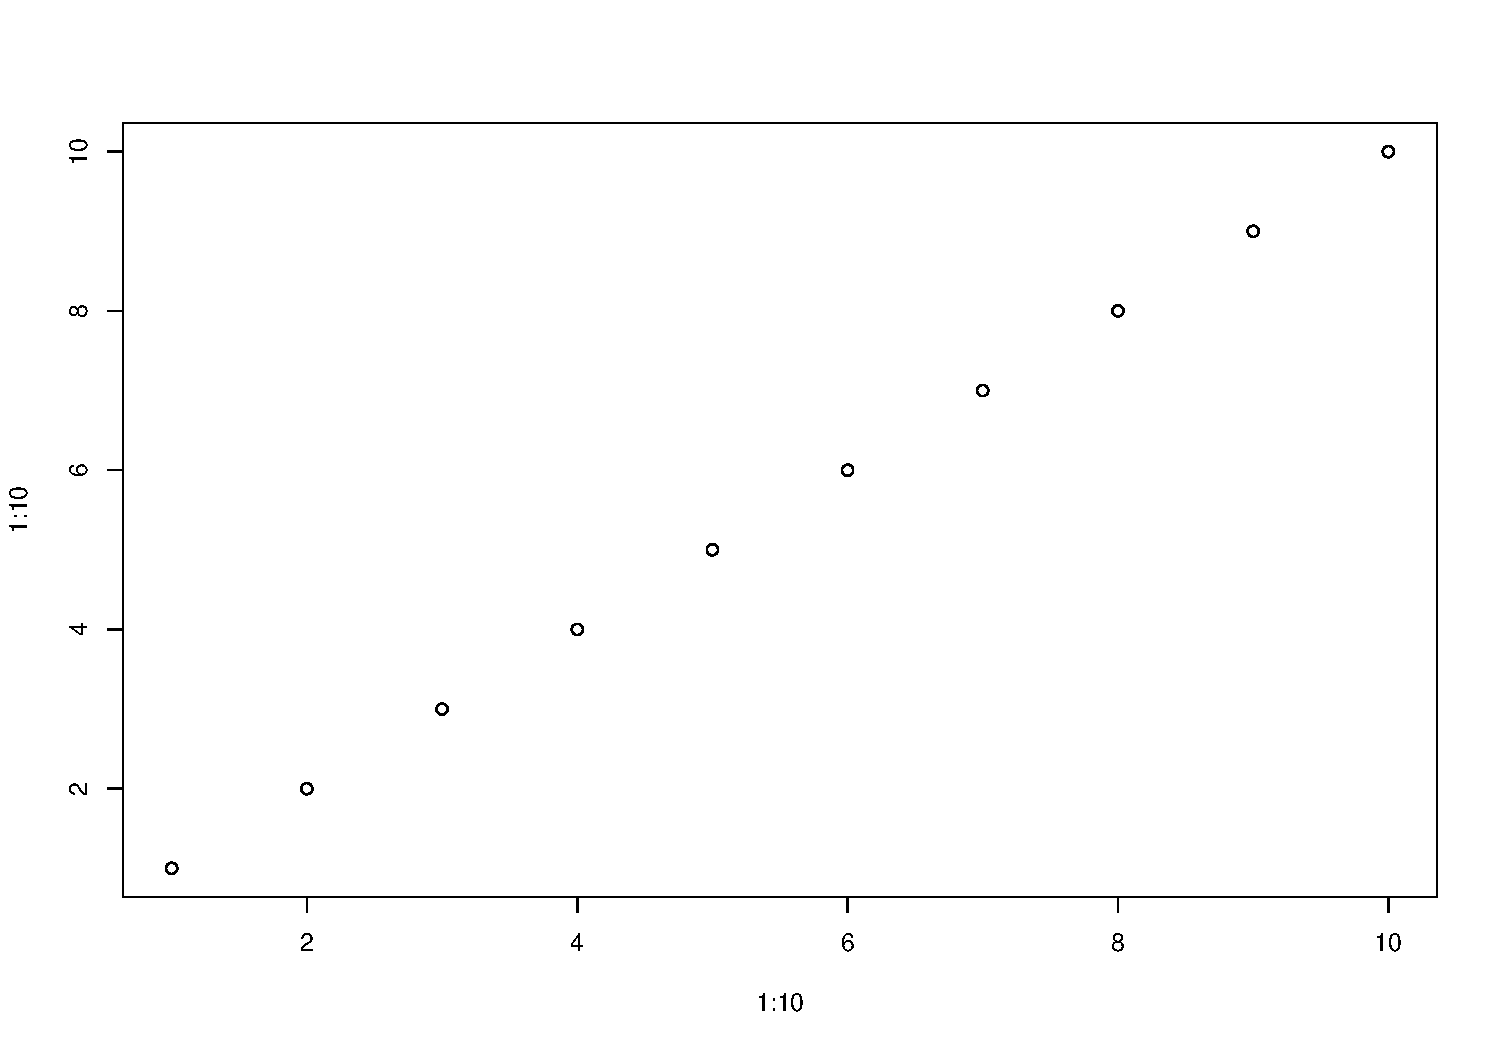
\includegraphics[width=1\linewidth]{AUTTheme_Rmd_Beamer_demo_files/figure-beamer/unnamed-chunk-4-1}
\end{column}

\begin{column}{0.4\textwidth}
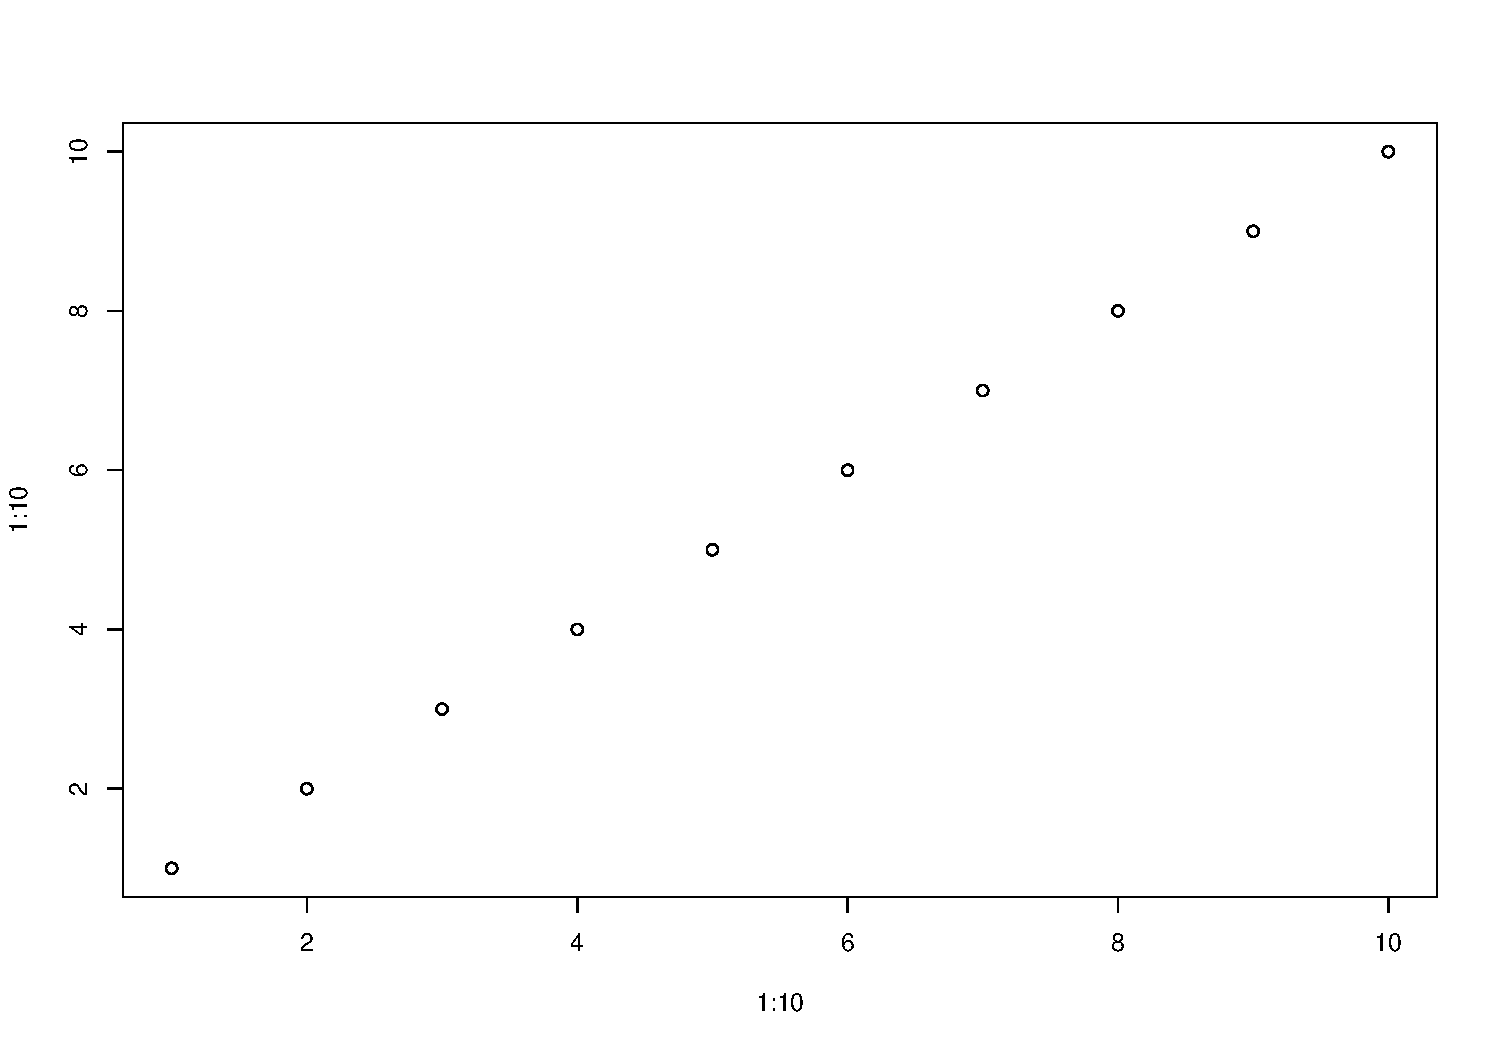
\includegraphics[width=1\linewidth]{AUTTheme_Rmd_Beamer_demo_files/figure-beamer/unnamed-chunk-5-1}
Column 2
\end{column}
\end{columns}
\end{frame}

\hypertarget{tables}{%
\subsection{Tables}\label{tables}}

\begin{frame}{Tables}
\begin{longtable}[]{@{}llll@{}}
\toprule()
\endhead
Assessment & Weighting & Hand out & Hand in \\
Quizzes & 15\% & Weekly & Weekly \\
Assignment & 25\% & Week 6 & Week 8 \\
Project & 60\% & Week 4 & Week 12 \\
Total & 100\% & & \\
\bottomrule()
\end{longtable}
\end{frame}

\hypertarget{latex-commands}{%
\section{LaTeX commands}\label{latex-commands}}

\hypertarget{overlays}{%
\subsection{Overlays}\label{overlays}}

\begin{frame}{Overlays}
This appears on all slides.
\only<2->{ \textbf{This only appears on slide 2}
}
\end{frame}

\hypertarget{footnotes}{%
\subsection{Footnotes}\label{footnotes}}

\begin{frame}{Footnotes}
There is a really good book about geometric processes. \footnote[frame]{
Lam, Yeh. The Geometric Process and Its Applications. World Scientific, Hackensack,
NJ, 2007.
} There is also a really good book about stochastic processes.
\footnote[frame]{
Ross, Sheldon. Stochastic Processes, 1998.
}
\end{frame}

\hypertarget{protecting-latex-commands}{%
\subsection{Protecting LaTeX commands}\label{protecting-latex-commands}}

\begin{frame}{Protecting LaTeX commands}
The following environment can be used to protect raw latex code (see
source)

\begin{tabular}{ll}
A & B \\
A & B \\
\end{tabular}
\end{frame}

\hypertarget{latex-environments}{%
\subsection{LaTeX Environments}\label{latex-environments}}

\begin{frame}{Example 1}
\protect\hypertarget{example-1}{}
For more information see
\url{https://bookdown.org/yihui/rmarkdown-cookbook/custom-blocks.html}

\begin{center}

\begin{minipage}{.5\linewidth}
This paragraph will be centered on the page, and its width is 50\% of
the width of its parent element.

\end{minipage}

\end{center}
\end{frame}

\end{document}
